\documentclass[10pt, letter]{article}
\newcommand{\doctitle}{%
CS 4649/7649: RIP - Robot Intelligence - Planning}
\newcommand{\bigO}{\ensuremath{\mathcal{O}}}
\usepackage{graphicx}
\usepackage{float}
\usepackage{comment}
\usepackage{fancyvrb}
\usepackage{booktabs}
\usepackage[usenames,dvipsnames]{color}
\usepackage[center]{caption}
\usepackage{algorithm}
\usepackage[T1]{fontenc}
\usepackage{algpseudocode}
\usepackage[margin=1in]{geometry}
\usepackage[usenames,dvipsnames]{color}
\usepackage{hyperref}
\usepackage{xcolor}
\usepackage{amsmath}
\hypersetup{
  colorlinks,
  citecolor=Violet,
  linkcolor=Black,
  urlcolor=Blue}
%------------------------Included every possible package we might need ------------------------%
\begin{document}
\title{\textbf{\doctitle} \\\textsc{Project 1: Classical Sokoban Planner}}
  \author {Arvind Krishnaa Jagannathan, Zheng Yong, Luis Gustavo, Zhengyi Hu}%Others please check your names here
   \date{}
\maketitle

\section{Pre-Project: Towers of Hanoi}
\subsection*{Planners Used}
The two classical planners which we are using for the Towers of Hanoi problem are the Blackbox planner \cite{kautz1998blackbox} (downloaded from \url{http://www.cs.rochester.edu/~kautz/satplan/blackbox/blackbox-download.html}) and the FF planner \cite{hoffmann2001fast} (downloaded from \url{http://fai.cs.uni-saarland.de/hoffmann/ff/FF-v2.3.tgz}). The definition of the Towers of Hanoi domain, as well as the representation of the initial state of the problem (from Figure \ref{fig1}) are in the corresponding PDDL files, namely \textit{hanoi-domain.pddl} and \textit{hanoi-3.pddl}.

\begin{figure}[h!]
  \centering
    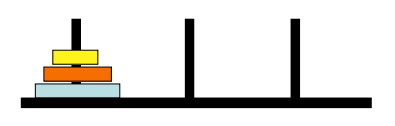
\includegraphics[scale = 0.3]{images/hanoi1}
    \caption{Towers of Hanoi with 3 disks}
  \label{fig1}
\end{figure}

\bibliographystyle{unsrt}
\bibliography{myrefs}
\end{document}